\documentclass[12pt]{report}
\usepackage[utf8]{inputenc}
\usepackage{geometry}
\usepackage{graphicx}
\geometry{margin=0.7in}

\title{CSC209 A3}
\author{Varak Tanashian \and Ethan Brook}
\date{\today}

\begin{document}
\maketitle
\tableofcontents
\newpage

\chapter{Project Overview}

% 1: Project Overview

This is just the template for now. More details once the project is done.

\chapter{Build Instructions}

% 2: Build Instructions

\textbf{Dependencies Required:}
\begin{itemize}
    \item \texttt{libavcodec-dev}, \texttt{libavformat-dev}, \texttt{libavutil-dev}, \texttt{libswscale-dev}, \texttt{libswresample-dev} (FFmpeg)
    \item \texttt{libsdl2-dev} (SDL2)
    \item \texttt{libgtk-3-dev} (GTK+3)
\end{itemize}

\textbf{To build:} 
Run \texttt{make} in the root directory.

\textbf{To run:}
Run \texttt{./vp}.

\chapter{Architecture Diagram}

% 3: Architecture Diagram

\begin{figure}[h!]
\centering
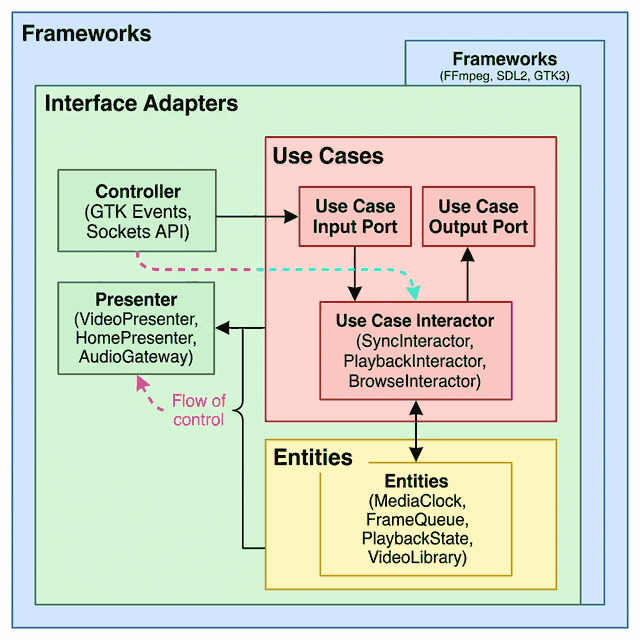
\includegraphics[width=0.8\textwidth]{imgs/architecture-diagram.png}
\caption{Overall project architecture.}
\end{figure}

\chapter{Communication Protocol}

% 4: Communication Protocol

For each message type, describe:
\begin{itemize}
    \item Sender and receiver
    \item Encoding
    \item Semantics / invariants
    \item Error handling
\end{itemize}

\chapter{Concurrency Model}

% 5: Concurrency Model

"Explain how your application handles concurrency:"
\begin{itemize}
    \item Forking and process coordination (Category 1)
    \item Select loops and fd sets (Category 2)
    \item How blocking is avoided
\end{itemize}

\chapter{Error Handling and Robustness}

% 6: Error Handling and Robustness

Describe at least three runtime error scenarios and how your code handles each. Example:
\begin{itemize}
    \item Client disconnects mid-message
    \item Writing to a closed pipe
    \item Malformed command input
\end{itemize}

\chapter{Team Contributions}
% 7: Team Contributions
Briefly list each team member and their specific contributions.

\end{document}
